\section{Análisis comparativo}

En las secciones anteriores pudimos ver el desempeño de cada filtro por separado. Veamos ahora la comparativa utilizando las medidas PESQ y STOI. En la figura \ref{fig:ch8_pesq_comparison} podemos ver la medida PESQ - Filtrada, tanto para el filtro adaptativo como para el filtro neuronal, para los distintos niveles de ruidos utilizados.

\begin{figure}[h]
	\centering
	\centerline{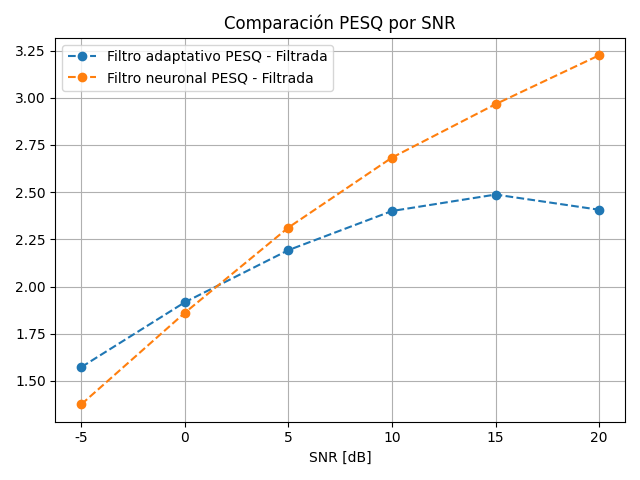
\includegraphics[scale=0.75]{images/ch8/comparison_pesq_by_snr.png}}
	\caption{Comparación PESQ en función de la SNR.}
	\label{fig:ch8_pesq_comparison_by_snr}
\end{figure}

Podemos ver en la figura \ref{fig:ch8_pesq_comparison_by_snr} que a altos niveles de ruido (SNR bajos), el desempeño del filtro adaptativo fue levemente superior, sin embargo a partir de los $\SI{5}{dB}$ el filtro neuronal superó al filtro adaptativo.	

En la figura \ref{fig:ch8_stoi_comparison_by_snr} podemos ver la medida STOI - Filtrada, tanto para el filtro adaptativo como para el filtro neuronal, para los distintos niveles de ruidos utilizados.

\begin{figure}[H]
	\centering
	\centerline{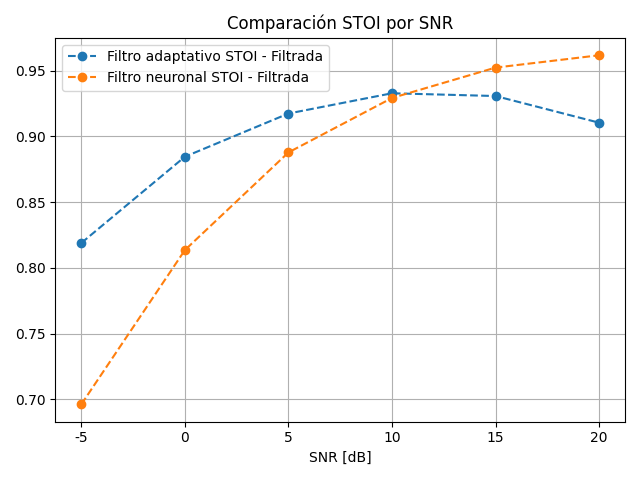
\includegraphics[scale=0.75]{images/ch8/comparison_stoi_by_snr.png}}
	\caption{Comparación STOI en función de la SNR.}
	\label{fig:ch8_stoi_comparison_by_snr}
\end{figure}

Para el caso de la STOI el filtro adaptativo fue superior en todos los casos. El filtro neuronal, a diferencia del adaptativo, trabaja en el dominio de la frecuencia lo cual lo hace mas susceptible a errores que generen una degradación en la inteligibilidad.